%%=============================================================================
%% Methodologie
%%=============================================================================

\chapter{Methodologie}
\label{ch:methodologie}

%% TODO: Hoe ben je te werk gegaan? Verdeel je onderzoek in grote fasen, en
%% licht in elke fase toe welke stappen je gevolgd hebt. Verantwoord waarom je
%% op deze manier te werk gegaan bent. Je moet kunnen aantonen dat je de best
%% mogelijke manier toegepast hebt om een antwoord te vinden op de
%% onderzoeksvraag.

In dit hoofdstuk worden eerst het doel en de systeemvereisten van de proof-of-concept besproken. Vervolgens wordt de selectie van technologieën voor de proof-of-concept behandeld, inclusief de keuze van de tabelstransformatie-algoritme(n). Uiteindelijk wordt de evaluatiessyteem verduidelijkt die gebruikt wordt om de performantie van de proof-of-concept te beoordelen.

\section{Systeemvereisten}
\label{sec:systeemvereisten}

\subsection{Goals}

Om een proof-of-concept succesvol te kunnen realiseren, moeten de volgende einddoelen hiervoor bereikt worden:

\begin{itemize}
    \item Een end-to-end-systeem dient gecreëerd te worden. Dit betekent dat de proof-of-concept niet enkel een tabeldetectiecomponent moet bevatten, maar eveneens een tabelstructuuranalysecomponent, een GUI en andere nodige elementen om de tabeltransformatie zoveel mogelijk te automatiseren.\\

    \item De software moet modulair geïmplementeerd worden. Code geschreven voor tabeldetectie, bijvoorbeeld, mag niet afhankelijk zijn van code geschreven voor tabelstructuuranalyse en vice versa. Dit maakt het mogelijk om later één deel van de tabeltransformatiesoftware te verbeteren of opnieuw te herschrijven, zonder hierdoor een impact te hebben op de rest van de software.\\

    \item Enkel open source software en libraries, zonder commercële restricties, mogen gebruikt worden.\\

    \item De proof-of-concept moet kunnen functioneren op verschillende eenvoudige tabellayouts. D.w.z. dat de tabeltransformatie niet mag afhangen van de fysieke dimensies van de tabel zelf of van de cellen. Noch mag het afhankelijk zijn van het aantal rijen of kolommen. Verder moet de software contextonafhankelijk zijn; een voedingswaardetabel bijvoorbeeld moet even nauwkeurig getransformeerd kunnen worden als een medicatieschema.\\

    \item Een tabeltransformatie moet kunnen uitgevoerd worden door een \Gls{REST}-server op te roepen. De tabeltransformatieresultaat die de server bij deze terug zal geven, moet een intuïtief, goed opgesteld \Gls{JSON}-object zijn.
\end{itemize}

\subsection{Non-goals}

Naast einddoelen die de scope van de proof-of-concept vormen zijn er eveneens non-goals, vereisten die expliciet buiten de scope liggen:

\begin{itemize}
    \item Het is niet de bedoeling om een volledige softwarepakket te ontwikkelen, met error handling, unit tests, integratie tests, authenticatie en meer.\\

    \item De proof-of-concept moet niet complexe tabellen kunnen verwerken. Hiermee worden voornamelijk tabellen bedoelt met meerdere niveau's van rijen en kolommen of tabellen met subtabellen.\\

    \item Preprocessing van de inputafbeeldingen wordt niet uitgevoerd. Er wordt verwacht dat de documenten correct zijn ingescand.\\

    \item Tabellen met handgeschreven tekst worden niet in beschouwing genomen.
\end{itemize}

\section{Selectie technologieën}
\label{sec:selectie-technologieën}

Op basis van de literatuurstudie (\autoref{ch:stand-van-zaken}) en de systeemvereisten (\autoref{sec:systeemvereisten}) kan de selectie van algoritmes en technologieën plaatsvinden.

\subsection{Tabeldetectie en Tabelstructuuranalyse}

De verschillende algoritmes voor tabeldetectie en tabelstructuuranalyse, behandeld in de literatuurstudie (\autoref{ch:stand-van-zaken}), hebben elk hun voor- en nadelen. Deze voor- en nadelen worden in de volgende tabel \ref{tab:voor-en-nadelen-tabel-transformatie-technieken} weergegeven.

\begin{table}[H]
\centering
\begin{tabular}{@{}lccc@{}}
\toprule
                            & Werkt zonder lijnen & Bruikbaar op afbeelding & Diverse layouts \\ \bottomrule
\multicolumn{4}{c}{\textit{Tabeldetectie}}                                                    \\ \toprule
\citeauthor{Watanabe1991}   &                     & \checkmark              & \checkmark      \\ \midrule
\citeauthor{Laurentini1992} &                     & \checkmark              & \checkmark      \\ \midrule
\citeauthor{Pyreddy1997}    & \checkmark          &                         & \checkmark      \\ \midrule
\citeauthor{Kieninger2001}  & \checkmark          & \checkmark              &                 \\ \midrule
\citeauthor{Cesarini2002}   &                     & \checkmark              & \checkmark      \\ \midrule
\citeauthor{Mandal2006}     & \checkmark          & \checkmark              &                 \\ \midrule
\citeauthor{Silva2009}      &                     &                         & \checkmark      \\ \midrule
\citeauthor{Kasar2013}      &                     & \checkmark              & \checkmark      \\ \midrule
\citeauthor{Fan2015}        & \checkmark          & \checkmark              & \checkmark      \\ \midrule
\citeauthor{Tran2015}       & \checkmark          & \checkmark              & \checkmark      \\ \midrule
\citeauthor{Hao2016}        &                     &                         &                 \\ \midrule
\citeauthor{Rashid2017}     & \checkmark          & \checkmark              &                 \\ \midrule
\citeauthor{Gilani2017}     & \checkmark          & \checkmark              & \checkmark      \\ \midrule
\citeauthor{Siddiqui2018}   & \checkmark          & \checkmark              & \checkmark      \\ \bottomrule
\multicolumn{4}{c}{\textit{Tabelstructuuranalyse}}                                            \\ \toprule
\citeauthor{Nazemi2016}     &                     & \checkmark              & \checkmark      \\ \midrule
\citeauthor{Qasim2019}      & \checkmark          & \checkmark              & \checkmark      \\ \bottomrule
\multicolumn{4}{c}{\textit{End-to-end-systemen}}                                              \\ \toprule
\citeauthor{Green1996}      &                     & \checkmark              &                 \\ \midrule
\citeauthor{Oro2009}        & \checkmark          &                         & \checkmark      \\ \midrule
\citeauthor{Schreiber2017}  & \checkmark          & \checkmark              & \checkmark      \\ \midrule
\citeauthor{Prasad2020}     & \checkmark          & \checkmark              & \checkmark      \\ \bottomrule
\end{tabular}
\caption{Voor- en nadelen van tabeltransformatiealgoritmes}
\label{tab:voor-en-nadelen-tabel-transformatie-technieken}
\end{table}

Wat tabeldetectie betreft, bieden de algoritmes \autocite{Tran2015}, \autocite{Gilani2017} en \autocite{Siddiqui2018} alle voordelen aan. Alle drie technieken werken zonder de aanwezigheid van horizontale of verticale tabelscheidingslijnen. Ze kunnen direct gebruikt worden op afbeeldingen, en zijn dus niet afhankelijk van PDF-metadata bijvoorbeeld. Tenslotte kunnen ze tabellen van verschillende layouts detecteren.

Van de technieken voor tabelstructuuranalyse heeft \autocite{Qasim2019} alle voordelen.

Tenslotte bieden de end-to-end-technieken, \autocite{Schreiber2017} en \autocite{Prasad2020}, eveneens alle voordelen.

Om het aantal kandidaatalgoritmes voor de proot-of-concept verder te verminderen, worden hun performanties met elkaar vergeleken. Omdat voor de tabelstructuuranalyse geen algoritmes te vinden zijn wiens performantiemeting met dezeflde methodologie uitgevoerd is, worden deze performanties niet in rekening gehouden. In onderstaande tabel \ref{tab:tabel-detectie-performanties} kan men de performantie van de verschillende technieken voor tabeldetectie terugvinden.

\begin{table}[H]
\centering
\begin{tabular}{@{}lccc@{}}
\toprule
                           & \Gls{Recall} & \Gls{Precisie} & \Gls{F1-score} \\ \midrule
\citeauthor{Tran2015}      & 0,9636       & 0,9521         & 0,9578         \\ \midrule
\citeauthor{Gilani2017}    & 0,9067       & 0,8230         & 0,8629         \\ \midrule
\citeauthor{Siddiqui2018}  & 0,996        & 0,996          & 0,996          \\ \midrule
\citeauthor{Schreiber2017} & 0,9615       & 0,9740         & 0,9677         \\ \midrule
\citeauthor{Prasad2020}    & 1,0          & 1,0            & 1,0            \\ \bottomrule
\end{tabular}
\caption{Tabeldetectieperformanties van de verschillende algoritmes}
\label{tab:tabel-detectie-performanties}
\end{table}

Deze performantiemetingen werden uitgevoerd op de \citefield{Gobel2013}{title} dataset. Dit is één van de meest bekende datasets voor tabeldetectie en tabelstructuuranalyse. Het bevat in totaal 238 ingescande documenten. Voor de berekening van de \Gls{F1-score} wordt bij deze dataset een \Gls{IoU} threshold van 0,5 gebruikt.

Aangezien de tabeldetectiealgoritme van \textcite{Prasad2020} de meest performante is, wordt deze geselectioneerd als de tabeldetectiecomponent van de proof-of-concept. Voor de tabelstructuuranalyse kan men nog kiezen tussen \autocite{Qasim2019}, \autocite{Schreiber2017} en opnieuw \autocite{Prasad2020}. Hoewel \autocite{Qasim2019} en \autocite{Schreiber2017} gepaste keuzes zijn, wordt er beslist om voor de structuuranalyse eveneens \autocite{Prasad2020} te selectioneren. Dit komt voornamelijk omdat \textcite{Prasad2020} niet enkel hun volledige modeltrainingdataset maar ook de code-implementatie van hun algoritme openbaar hebben gemaakt, met een open source licentie.

\subsection{Programmeertaal}

Voor de programmeertaal van de proof-of-concept wordt Python \autocite{VanRossum2009} gekozen, en dit voor verschillende redenen:

\begin{itemize}
    \item Python is een multifunctioneel programmeertaal die toelaat om eenvoudig en snel softwareprototypes te creëren.\\

    \item Het heeft een grote bibliotheek van libaries voor onder meer statistiek en data-analyse, zoals Numpy \autocite{Oliphant2006} en Pandas \autocite{McKinney2010}.\\

    \item De open source code van \textcite{Prasad2020} is reeds in Python geschreven. Door met Python verder te werken, kan code herbruikt worden en zal een een volledig nieuwe reïmplementatie van de software dus niet nodig worden.
\end{itemize}

\subsection{Interne tabelmodel}

Om de getransformeerd tabel te kunnen verwerken en verbeteren, moet de software van de proof-of-concept deze d.m.v. een datastructuur bijhouden. Hoewel voor de datastructuur JSON of XML gekozen kan worden, wordt er beslist om intern de getransformeerd tabel te presenteren en te verwerken d.m.v. een Pandas Dataframe. Een Pandas Dataframe is een twee dimensionele tabulaire datastructuur van de Pandas library. Deze datastructuur bestaat voornamelijk uit drie hoofdcomponenten, die in onderstaande figuur worden weergegeven: rijen, kolommen en data.

\begin{figure}[H]
    \centering
    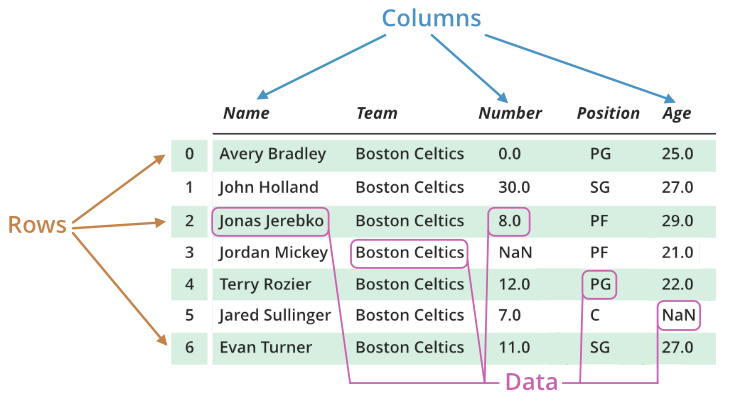
\includegraphics[width=0.8\textwidth]{img/pandas_dataframe.png}
    \caption{Anatomie van een Pandas Dataframe. Bron: \textcite{GeeksforGeeks2020}}
    \label{fig:anatomie-pandas-dataframe}
\end{figure}

Niet enkel modelleert een Pandas Dataframe, met zijn twee dimensionele structuur, op een gepaste manier een tabel maar het bezit eveneens andere voordelen. Zo kan de opgeslagen data heterogeen zijn, d.w.z. dat de datatypes van de data-elementen niet identiek hoeven te zijn. Verder bezit het meerdere functionaliteiten om data eenvoudig te manipuleren. Tenslotte kan een Pandas dataframe zeer efficiënt met grote hoeveelheden data werken.

\subsection{\Gls{OCR}}

Voor de \Gls{OCR}-component zijn er niet veel keuzes. Tesseract \autocite{Kay2007} is momenteel de enige \Gls{OCR}-software die open source is en nauwkeurig tekst in afbeeldingen detecteert en transformeert. Bovendien kan de Python library, Pytesseract \autocite{Lee2009}, gebruikt worden om Tesseract-functionaliteiten met Python te gebruiken. Zo kan men Tesseract functionaliteiten d.m.v. Pytesseract in Python code oproepen en kunnen de \Gls{OCR}-resultaten als een Pandas Dataframe verkregen worden.

\subsection{Back end server}

Voor de \Gls{REST}-server wordt Flask \autocite{Grinberg2018} gekozen. Flask is een eenvoudige micro web framework, bedoeld voor Python-softwareontwikkeling, met \Gls{REST}-ondersteuning.

\subsection{Front end}

Er bestaan verschillende front end frameworks om snel en eenvoudig GUI's te ontwerpen die via de browser gebruikt zullen kunnen worden, zoals Angular \autocite{Jain2014} en React \autocite{Fedosejev2016}. Voor deze proof-of-concept wordt React gebruikt, in combinatie met de UI framework Ant Design \autocite{Financial2020}. De UI framework Ant Design biedt herbruikbare UI-componenten, onder meer voor tabulair data, die de ontwikkeling van de proof-of-concept vereenvoudigen en versnellen.

\section{Performantiemeting}
\label{sec:performantie-meting}

De architectuur van de proof-of-concept wordt in de volgende hoofdstuk \ref{ch:proof-of-concept} meer in detail besproken. Om de performantie van de software te kunnen meten, wordt de software van de proof-of-concept uitgevoerd op dertig willekeurige ingescande documenten waarin in elk document één of meerdere tabelafbeeldingen te vinden zijn. Het resultaat van de tabeltransformatie op deze testdocumenten worden in hoofdstuk \ref{ch:resultaten} behandeld.
